

\documentclass[12pt]{report}
\usepackage[utf8]{inputenc}
\usepackage[russian]{babel}
\usepackage[14pt]{extsizes}
\usepackage{listings}
\usepackage{graphicx}
\usepackage{amsmath,amsfonts,amssymb,amsthm,mathtools} 
\usepackage{pgfplots}
\usepackage{filecontents}
\usepackage{float}
\usepackage{indentfirst}
\usepackage{eucal}
\usepackage{enumitem}
%s\documentclass[openany]{book}
\frenchspacing

\usepackage{titlesec}
\titleformat{\section}
{\normalsize\bfseries}
{\thesection}
{1em}{}
\titlespacing*{\chapter}{0pt}{-30pt}{8pt}
\titlespacing*{\section}{\parindent}{*4}{*4}
\titlespacing*{\subsection}{\parindent}{*4}{*4}

\usepackage{indentfirst} % Красная строка

\usetikzlibrary{datavisualization}
\usetikzlibrary{datavisualization.formats.functions}

\usepackage{amsmath}


% Для листинга кода:
\lstset{ %
	language=python,                 % выбор языка для подсветки (здесь это С)
	texcl=true,
	extendedchars=\true,
	basicstyle=\small\sffamily, % размер и начертание шрифта для подсветки кода
	numbers=left,               % где поставить нумерацию строк (слева\справа)
	numberstyle=\tiny,           % размер шрифта для номеров строк
	stepnumber=1,                   % размер шага между двумя номерами строк
	numbersep=5pt,                % как далеко отстоят номера строк от подсвечиваемого кода
	showspaces=false,            % показывать или нет пробелы специальными отступами
	showstringspaces=false,      % показывать или нет пробелы в строках
	showtabs=false,             % показывать или нет табуляцию в строках
	frame=single,              % рисовать рамку вокруг кода
	tabsize=2,                 % размер табуляции по умолчанию равен 2 пробелам
	captionpos=t,              % позиция заголовка вверху [t] или внизу [b] 
	breaklines=true,           % автоматически переносить строки (да\нет)
	breakatwhitespace=false, % переносить строки только если есть пробел
	escapeinside={\#*}{*)}   % если нужно добавить комментарии в коде
}


\usepackage[left=2cm,right=2cm, top=2cm,bottom=2cm,bindingoffset=0cm]{geometry}
% Для измененных титулов глав:
\usepackage{titlesec, blindtext, color} % подключаем нужные пакеты
\definecolor{gray75}{gray}{0.75} % определяем цвет
\newcommand{\hsp}{\hspace{20pt}} % длина линии в 20pt
% titleformat определяет стиль
\titleformat{\chapter}[hang]{\Huge\bfseries}{\thechapter\hsp\textcolor{gray75}{|}\hsp}{0pt}{\Huge\bfseries}


% plot
\usepackage{pgfplots}
\usepackage{filecontents}
\usetikzlibrary{datavisualization}
\usetikzlibrary{datavisualization.formats.functions}

\begin{document}
	%\def\chaptername{} % убирает "Глава"
	\thispagestyle{empty}
	\begin{titlepage}
		\noindent \begin{minipage}{0.15\textwidth}
			
\includegraphics[width=\linewidth]{img/b_logo}
		\end{minipage}
		\noindent\begin{minipage}{0.9\textwidth}\centering
			\textbf{Министерство науки и высшего образования Российской Федерации}\\
			\textbf{Федеральное государственное бюджетное образовательное учреждение высшего образования}\\
			\textbf{~~~«Московский государственный технический университет имени Н.Э.~Баумана}\\
			\textbf{(национальный исследовательский университет)»}\\
			\textbf{(МГТУ им. Н.Э.~Баумана)}
		\end{minipage}
		
		\noindent\rule{18cm}{3pt}
		\newline\newline
		\noindent ФАКУЛЬТЕТ $\underline{\text{«Информатика и системы управления»}}$ \newline\newline
		\noindent КАФЕДРА $\underline{\text{«Программное обеспечение ЭВМ и информационные технологии»}}$\newline\newline\newline
		
		\begin{center}
			\noindent\begin{minipage}{1.1\textwidth}\centering
				\Large\textbf{  Отчет по лабораторной работе №1}\newline
				\textbf{по дисциплине <<Моделирование>>}\newline
			\end{minipage}
		\end{center}
		
		\noindent\textbf{Тема} $\underline{\text{Программная реализация приближенного аналитического метода и}}$\newline   
		$\underline{\text{		численных алгоритмов первого и второго порядков точности при}}$\newline
		$\underline{\text{решении задачи Коши для ОДУ}}$\newline\newline
		\noindent\textbf{Студент} $\underline{\text{Зайцева А. А.~~~~~~~~~~~~~~~~~~~~~~~~~~~~~~~~~~~~~~~~~~}}$\newline\newline
		\noindent\textbf{Группа} $\underline{\text{ИУ7-62Б~~~~~~~~~~~~~~~~~~~~~~~~~~~~~~~~~~~~~~~~~~~~~~~~~~}}$\newline\newline
		\noindent\textbf{Оценка (баллы)} $\underline{\text{~~~~~~~~~~~~~~~~~~~~~~~~~~~~~~~~~~~~~~~~~~~~~~~~~}}$\newline\newline
		\noindent\textbf{Преподаватель} $\underline{\text{Градов В. М.~~~~~~~~~~~~~~~~~~~~~~~~~~~~}}$\newline\newline\newline
		
		\begin{center}
			\vfill
			Москва~---~\the\year
			~г.
		\end{center}
	\end{titlepage}

\chapter{Задание}

\textbf{Цель работы.} 

Получение навыков решения задачи Коши для ОДУ методами Пикара и явными методами первого порядка точности (Эйлера) и второго порядка точности (Рунге-Кутты).

\textbf{Исходные данные.} 

ОДУ \ref{eq:task1}, не имеющее аналитического решения:

\begin{equation}
	{\begin{cases}
			u'(x) = u^2 + x^2 \\
			u(0) = 0.
	\end{cases}}
	\label{eq:task1}
\end{equation}

\textbf{Результат работы программы.}

1. Таблица, содержащая значения аргумента с заданным шагом в интервале [0, xmax] и результаты расчета функции u(x) в приближениях Пикара (от 1-го до 4-го), а также численными методами. Границу интервала xmax выбирать максимально возможной из условия, чтобы численные методы обеспечивали точность вычисления решения уравнения u(x) до второго знака после запятой.

2. График функции в диапазоне [-xmax, xmax].

\chapter{Теоретическая часть}

Обыкновенное дифференциальное уравнение (ОДУ) n-ого порядка имеет вид \ref{eq:ody}:

\begin{equation}
	F(x, u', u'', ... , u^{(n)} = 0)
	\label{eq:ody}.
\end{equation}

Задача Коши состоит в нахождении решения дифференциального уравнения, удовлетворяющего начальным условиям \ref{eq:ref1}:


\begin{equation}
	{\begin{cases}
			u'(x) = f(x,u) \\
			u(\xi) = \eta
	\end{cases}}
	\label{eq:ref1}
\end{equation}

Рассмотрим методы решения этой задачи.

%Методы решения ОДУ в задачи Коши:

%\begin{enumerate}
%	\item аналитические;
%	\item приближенно аналитические;
%	\item численные.
%\end{enumerate}

\section{Метод Пикара}

Метод Пикара является приближенно-аналитическим. Идея состоит в том, чтобы заменить дифференциальное уравнение интегральным \ref{eq:ref2}:.


\begin{equation}
	y^{s}(x) = \eta + \int_{\xi}^{x} f(t, y^{s-1}(t)) dt
	\label{eq:ref2}
\end{equation}

\begin{equation}
	y^{(0)} = \eta
\end{equation}

%Метод сходится если правая часть непрерывна и выполнено условие Липшица: $|f(x, u_1) - f(x, u_2)| \leq L |u_1-u_2|$, где L - константа Липшица. 

Для данного в задании ОДУ \ref{eq:task1}:

\begin{equation}
	y^{(1)} = 0 + \int_{0}^{x} t^2 dt= \frac{x^3}{3} 
\end{equation}

\begin{equation}
	y^{(2)} = 0 + \int_{0}^{x}\left[ \left( t^2 + \frac{t^3}{3} \right)^2 \right] dt = \frac{x^3}{3} + \frac{x^7}{63}
\end{equation}

\begin{equation}
	\begin{split}
		y^{(3)} = 0 + \int_{0}^{x}\left[t^2 + \left(\frac{t^7}{63} + \frac{t^3}{3} \right)^2\right] dt = \\ 
		\frac{x^3}{3} + \frac{x^7}{63} + \frac{2x^{11}}{2079} + \frac{x^{15}}{59535}
	\end{split}
\end{equation}

\begin{equation}
	\begin{split}
		y^{(4)} = 0 + \int_{0}^{x}\left[t^2 + \left( \frac{t^3}{3} + \frac{t^7}{63} + \frac{2t^{11}}{2079} + \frac{t^{15}}{59535} \right)^2 \right] dt = \\ 
		= \frac{x^3}{3} + \frac{x^{7}}{63} + \frac{2x^{11}}{2079} + \frac{13x^{15}}{218295} + \frac{82x^{19}}{37328445} + \\
		+ \frac{662x^{23}}{10438212015} + \frac{4x^{27}}{3341878155} + \frac{x^{31}}{109876902975}
	\end{split}
\end{equation}

\section{Метод Эйлера}
Метод Эйлера -- это явный (численный) метод первого порядка точности, использующий формулу \ref{eq:ref3}:

\begin{equation}
	y_{n+1} = y_n + h*f(x_n, y_n).
	\label{eq:ref3}
\end{equation}


\section{Метод Рунге-Кутты}

Метод Ругнге-Кутты -- это явный (численный) метод второго порядка точности, использующий формулу \ref{eq:ref4}:

%\begin{equation}
	%y_{n+1} = y_n + %h*[\frac{k_1}{2} + %\frac{k_2}{2}],
%	\label{eq:ref4}
%\end{equation}
%где $k_1 = f(x_n, y_n)$, $k_2 = f(x_n + h, y_n + hk_1)$.

\begin{equation}
	y_{n+1} = y_n + h*[(1-\alpha)k_1 + \alpha * k_2],
	\label{eq:ref4}
\end{equation}
где $k_1 = f(x_n, y_n)$, $k_2 = f(x_n + \frac{h}{2\alpha}, y_n + \frac{h}{2\alpha}k_1)$, $\alpha$ = 1 или $\frac{1}{2}$
 



\chapter{Исходный код алгоритмов}

\begin{lstlisting}[language=Python]
	class UDESolver:
		def __init__(self, x_start, y_start, x_max, step, f, f_derivatives):
			if (x_start < x_max) != (step > 0):
				raise ValueError('Ошибка в шаге')
	
		self.x_start = x_start
		self.y_start = y_start
		self.x_max = x_max
		self.step = step
		self.f = f
		self.f_derivativesf_derivatives = f_derivativesf_derivatives
		self.cmp_func = lambda x1, x2: x1 < x2 + EPS
	
		def reverse_move(self):
			self.step *= -1
			self.x_max *= -1
			self.cmp_func = lambda x1, x2: x1 > x2 - EPS
		
		def x_range(self):
			result = []
			x = self.x_start
			while self.cmp_func(x, self.x_max):
				result.append(x)
				x += self.step
			return result
		
			def solve_euler(self):
			result = []
			x, y = self.x_start, self.y_start
			
			while self.cmp_func(x, self.x_max):
				result.append(y)
			
				y = y + self.step * self.f(x, y)
				x += self.step
			
			return result
		
		def solve_runge_kutta(self):
			a = 0.5
			result = []
			x, y = self.x_start, self.y_start
			
			while self.cmp_func(x, self.x_max):
				result.append(y)
			
				k1 = self.f(x, y)
				k2 = self.f(x + self.step / (2 * a), y + self.step * k1 / (2 * a))
				y += self.step * ((1 - a) * k1 + a * k2)
				x += self.step
			
			return result
		
		def solve_picar(self, approx):
			func = self.f_derivatives[approx - 1]
			result = []
			x, y = self.x_start, self.y_start
			
			while self.cmp_func(x, self.x_max):
				result.append(y)
				x += self.step
				y = func(x)
			
			return result
	
	
	def function(x, u):
		return x * x + u * u
	
	def fd1(x):
		return pow(x, 3) / 3
	
	
	def fd2(x):
		return fd1(x) + pow(x, 7) / 63
	
	
	def fd3(x):
		return fd2(x) + 2 * pow(x, 11) / 2079 + pow(x, 15) / 59535
	
	
	def fd4(x):
		return (fd2(x) + 2 * pow(x, 11) / 2079 + 13 * pow(x, 15) / 218295 +
		82 * pow(x, 19) / 37328445 + 662 * pow(x, 23) / 10438212015 +
		4 * pow(x, 27) / 3341878155 + pow(x, 31) / 109876902975)
\end{lstlisting}

%Приближение Пикара высчитывается по выведенной формуле:

%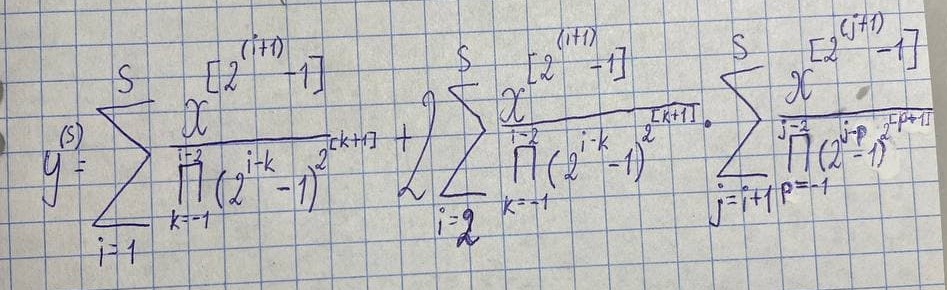
\includegraphics[scale=1]{img/formula}\label{fig:formula}

\chapter{Результат работы программы}

Исходные данные: h=$10^{-4}$, xmax = 1.77, x0=0, y0 = 0, округление при выводе - до 2 знака после запятой, шаг вывода=0.01.


На рисунке \ref{fig:plot} приведен график функции в диапазоне [-xmax; xmax].

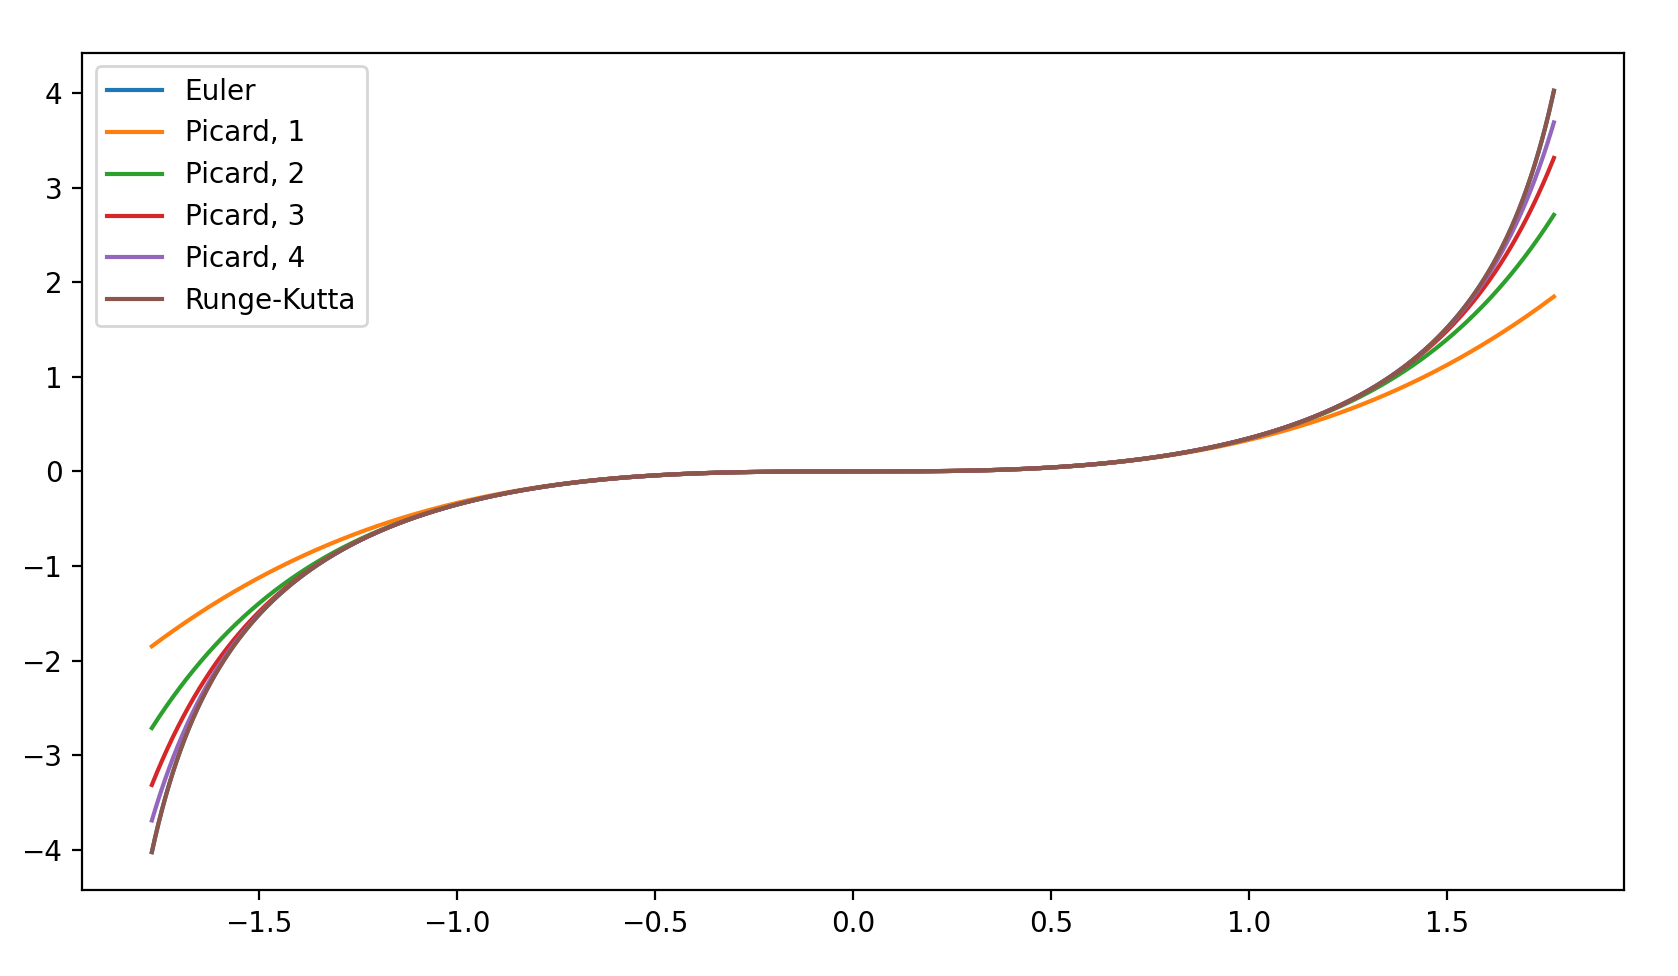
\includegraphics[scale=0.6]{img/plot}\label{fig:plot}

Ниже приведена таблица с полученными данным.

\begin{lstlisting}[language=Python]
x      Euler  Runge-Kutta  Picard, 1  Picard, 2  Picard, 3  Picard, 4
                                                                  
0.00   0.00         0.00       0.00       0.00       0.00       0.00
0.01   0.00         0.00       0.00       0.00       0.00       0.00
0.02   0.00         0.00       0.00       0.00       0.00       0.00
0.03   0.00         0.00       0.00       0.00       0.00       0.00
0.04   0.00         0.00       0.00       0.00       0.00       0.00
0.05   0.00         0.00       0.00       0.00       0.00       0.00
0.06   0.00         0.00       0.00       0.00       0.00       0.00
0.07   0.00         0.00       0.00       0.00       0.00       0.00
0.08   0.00         0.00       0.00       0.00       0.00       0.00
0.09   0.00         0.00       0.00       0.00       0.00       0.00
0.10   0.00         0.00       0.00       0.00       0.00       0.00
0.11   0.00         0.00       0.00       0.00       0.00       0.00
0.12   0.00         0.00       0.00       0.00       0.00       0.00
0.13   0.00         0.00       0.00       0.00       0.00       0.00
0.14   0.00         0.00       0.00       0.00       0.00       0.00
0.15   0.00         0.00       0.00       0.00       0.00       0.00
0.16   0.00         0.00       0.00       0.00       0.00       0.00
0.17   0.00         0.00       0.00       0.00       0.00       0.00
0.18   0.00         0.00       0.00       0.00       0.00       0.00
0.19   0.00         0.00       0.00       0.00       0.00       0.00
0.20   0.00         0.00       0.00       0.00       0.00       0.00
0.21   0.00         0.00       0.00       0.00       0.00       0.00
0.22   0.00         0.00       0.00       0.00       0.00       0.00
0.23   0.00         0.00       0.00       0.00       0.00       0.00
0.24   0.00         0.00       0.00       0.00       0.00       0.00
0.25   0.01         0.01       0.01       0.01       0.01       0.01
0.26   0.01         0.01       0.01       0.01       0.01       0.01
0.27   0.01         0.01       0.01       0.01       0.01       0.01
0.28   0.01         0.01       0.01       0.01       0.01       0.01
0.29   0.01         0.01       0.01       0.01       0.01       0.01
0.30   0.01         0.01       0.01       0.01       0.01       0.01
0.31   0.01         0.01       0.01       0.01       0.01       0.01
0.32   0.01         0.01       0.01       0.01       0.01       0.01
0.33   0.01         0.01       0.01       0.01       0.01       0.01
0.34   0.01         0.01       0.01       0.01       0.01       0.01
0.35   0.01         0.01       0.01       0.01       0.01       0.01
0.36   0.02         0.02       0.02       0.02       0.02       0.02
0.37   0.02         0.02       0.02       0.02       0.02       0.02
0.38   0.02         0.02       0.02       0.02       0.02       0.02
0.39   0.02         0.02       0.02       0.02       0.02       0.02
0.40   0.02         0.02       0.02       0.02       0.02       0.02
0.41   0.02         0.02       0.02       0.02       0.02       0.02
0.42   0.02         0.02       0.02       0.02       0.02       0.02
0.43   0.03         0.03       0.03       0.03       0.03       0.03
0.44   0.03         0.03       0.03       0.03       0.03       0.03
0.45   0.03         0.03       0.03       0.03       0.03       0.03
0.46   0.03         0.03       0.03       0.03       0.03       0.03
0.47   0.03         0.03       0.03       0.03       0.03       0.03
0.48   0.04         0.04       0.04       0.04       0.04       0.04
0.49   0.04         0.04       0.04       0.04       0.04       0.04
0.50   0.04         0.04       0.04       0.04       0.04       0.04
0.51   0.04         0.04       0.04       0.04       0.04       0.04
0.52   0.05         0.05       0.05       0.05       0.05       0.05
0.53   0.05         0.05       0.05       0.05       0.05       0.05
0.54   0.05         0.05       0.05       0.05       0.05       0.05
0.55   0.06         0.06       0.06       0.06       0.06       0.06
0.56   0.06         0.06       0.06       0.06       0.06       0.06
0.57   0.06         0.06       0.06       0.06       0.06       0.06
0.58   0.07         0.07       0.07       0.07       0.07       0.07
0.59   0.07         0.07       0.07       0.07       0.07       0.07
0.60   0.07         0.07       0.07       0.07       0.07       0.07
0.61   0.08         0.08       0.08       0.08       0.08       0.08
0.62   0.08         0.08       0.08       0.08       0.08       0.08
0.63   0.08         0.08       0.08       0.08       0.08       0.08
0.64   0.09         0.09       0.09       0.09       0.09       0.09
0.65   0.09         0.09       0.09       0.09       0.09       0.09
0.66   0.10         0.10       0.10       0.10       0.10       0.10
0.67   0.10         0.10       0.10       0.10       0.10       0.10
0.68   0.11         0.11       0.10       0.11       0.11       0.11
0.69   0.11         0.11       0.11       0.11       0.11       0.11
0.70   0.12         0.12       0.11       0.12       0.12       0.12
0.71   0.12         0.12       0.12       0.12       0.12       0.12
0.72   0.13         0.13       0.12       0.13       0.13       0.13
0.73   0.13         0.13       0.13       0.13       0.13       0.13
0.74   0.14         0.14       0.14       0.14       0.14       0.14
0.75   0.14         0.14       0.14       0.14       0.14       0.14
0.76   0.15         0.15       0.15       0.15       0.15       0.15
0.77   0.15         0.15       0.15       0.15       0.15       0.15
0.78   0.16         0.16       0.16       0.16       0.16       0.16
0.79   0.17         0.17       0.16       0.17       0.17       0.17
0.80   0.17         0.17       0.17       0.17       0.17       0.17
0.81   0.18         0.18       0.18       0.18       0.18       0.18
0.82   0.19         0.19       0.18       0.19       0.19       0.19
0.83   0.19         0.20       0.19       0.19       0.20       0.20
0.84   0.20         0.20       0.20       0.20       0.20       0.20
0.85   0.21         0.21       0.20       0.21       0.21       0.21
0.86   0.22         0.22       0.21       0.22       0.22       0.22
0.87   0.23         0.23       0.22       0.23       0.23       0.23
0.88   0.23         0.23       0.23       0.23       0.23       0.23
0.89   0.24         0.24       0.23       0.24       0.24       0.24
0.90   0.25         0.25       0.24       0.25       0.25       0.25
0.91   0.26         0.26       0.25       0.26       0.26       0.26
0.92   0.27         0.27       0.26       0.27       0.27       0.27
0.93   0.28         0.28       0.27       0.28       0.28       0.28
0.94   0.29         0.29       0.28       0.29       0.29       0.29
0.95   0.30         0.30       0.29       0.30       0.30       0.30
0.96   0.31         0.31       0.29       0.31       0.31       0.31
0.97   0.32         0.32       0.30       0.32       0.32       0.32
0.98   0.33         0.33       0.31       0.33       0.33       0.33
0.99   0.34         0.34       0.32       0.34       0.34       0.34
1.00   0.35         0.35       0.33       0.35       0.35       0.35
1.01   0.36         0.36       0.34       0.36       0.36       0.36
1.02   0.37         0.37       0.35       0.37       0.37       0.37
1.03   0.39         0.39       0.36       0.38       0.39       0.39
1.04   0.40         0.40       0.37       0.40       0.40       0.40
1.05   0.41         0.41       0.39       0.41       0.41       0.41
1.06   0.42         0.42       0.40       0.42       0.42       0.42
1.07   0.44         0.44       0.41       0.43       0.44       0.44
1.08   0.45         0.45       0.42       0.45       0.45       0.45
1.09   0.46         0.46       0.43       0.46       0.46       0.46
1.10   0.48         0.48       0.44       0.47       0.48       0.48
1.11   0.49         0.49       0.46       0.49       0.49       0.49
1.12   0.51         0.51       0.47       0.50       0.51       0.51
1.13   0.52         0.52       0.48       0.52       0.52       0.52
1.14   0.54         0.54       0.49       0.53       0.54       0.54
1.15   0.55         0.55       0.51       0.55       0.55       0.55
1.16   0.57         0.57       0.52       0.57       0.57       0.57
1.17   0.59         0.59       0.53       0.58       0.59       0.59
1.18   0.60         0.60       0.55       0.60       0.60       0.60
1.19   0.62         0.62       0.56       0.62       0.62       0.62
1.20   0.64         0.64       0.58       0.63       0.64       0.64
1.21   0.66         0.66       0.59       0.65       0.66       0.66
1.22   0.68         0.68       0.61       0.67       0.68       0.68
1.23   0.70         0.70       0.62       0.69       0.70       0.70
1.24   0.72         0.72       0.64       0.71       0.72       0.72
1.25   0.74         0.74       0.65       0.73       0.74       0.74
1.26   0.76         0.76       0.67       0.75       0.76       0.76
1.27   0.78         0.78       0.68       0.77       0.78       0.78
1.28   0.81         0.81       0.70       0.79       0.80       0.81
1.29   0.83         0.83       0.72       0.81       0.83       0.83
1.30   0.85         0.85       0.73       0.83       0.85       0.85
1.31   0.88         0.88       0.75       0.85       0.87       0.88
1.32   0.90         0.90       0.77       0.88       0.90       0.90
1.33   0.93         0.93       0.78       0.90       0.92       0.93
1.34   0.96         0.96       0.80       0.93       0.95       0.95
1.35   0.98         0.98       0.82       0.95       0.98       0.98
1.36   1.01         1.01       0.84       0.98       1.01       1.01
1.37   1.04         1.04       0.86       1.00       1.03       1.04
1.38   1.07         1.07       0.88       1.03       1.06       1.07
1.39   1.10         1.10       0.90       1.05       1.09       1.10
1.40   1.13         1.13       0.91       1.08       1.12       1.13
1.41   1.17         1.17       0.93       1.11       1.16       1.16
1.42   1.20         1.20       0.95       1.14       1.19       1.20
1.43   1.23         1.24       0.97       1.17       1.22       1.23
1.44   1.27         1.27       1.00       1.20       1.26       1.27
1.45   1.31         1.31       1.02       1.23       1.29       1.31
1.46   1.35         1.35       1.04       1.26       1.33       1.34
1.47   1.39         1.39       1.06       1.29       1.37       1.38
1.48   1.43         1.43       1.08       1.33       1.41       1.42
1.49   1.47         1.47       1.10       1.36       1.45       1.47
1.50   1.52         1.52       1.12       1.40       1.49       1.51
1.51   1.56         1.56       1.15       1.43       1.53       1.56
1.52   1.61         1.61       1.17       1.47       1.57       1.60
1.53   1.66         1.66       1.19       1.51       1.62       1.65
1.54   1.71         1.71       1.22       1.54       1.67       1.70
1.55   1.77         1.77       1.24       1.58       1.71       1.76
1.56   1.82         1.82       1.27       1.62       1.76       1.81
1.57   1.88         1.88       1.29       1.66       1.82       1.87
1.58   1.94         1.95       1.31       1.70       1.87       1.92
1.59   2.01         2.01       1.34       1.75       1.92       1.99
1.60   2.08         2.08       1.37       1.79       1.98       2.05
1.61   2.15         2.15       1.39       1.84       2.04       2.12
1.62   2.22         2.22       1.42       1.88       2.10       2.18
1.63   2.30         2.30       1.44       1.93       2.16       2.26
1.64   2.38         2.38       1.47       1.98       2.23       2.33
1.65   2.46         2.47       1.50       2.03       2.29       2.41
1.66   2.55         2.56       1.52       2.08       2.36       2.49
1.67   2.65         2.65       1.55       2.13       2.44       2.58
1.68   2.75         2.75       1.58       2.18       2.51       2.67
1.69   2.86         2.86       1.61       2.23       2.59       2.76
1.70   2.97         2.97       1.64       2.29       2.67       2.86
1.71   3.09         3.09       1.67       2.35       2.75       2.96
1.72   3.22         3.22       1.70       2.40       2.84       3.07
1.73   3.36         3.36       1.73       2.46       2.92       3.18
1.74   3.51         3.51       1.76       2.52       3.02       3.30
1.75   3.67         3.67       1.79       2.58       3.11       3.42
1.76   3.84         3.84       1.82       2.65       3.21       3.55
1.77   4.02         4.03       1.85       2.71       3.31       3.69
\end{lstlisting}

На рисунке \ref{fig:differences} приведен вывод программы при шагах 1e-4 (слева) и 1e-5 (справа). Порядок колонок сохранен. Нас интересуют первые 3 (справа и слева) -- значение аргумента, результат, вычисленный методом Эйлера и результат, вычисленный методом Рунге-Кутты.

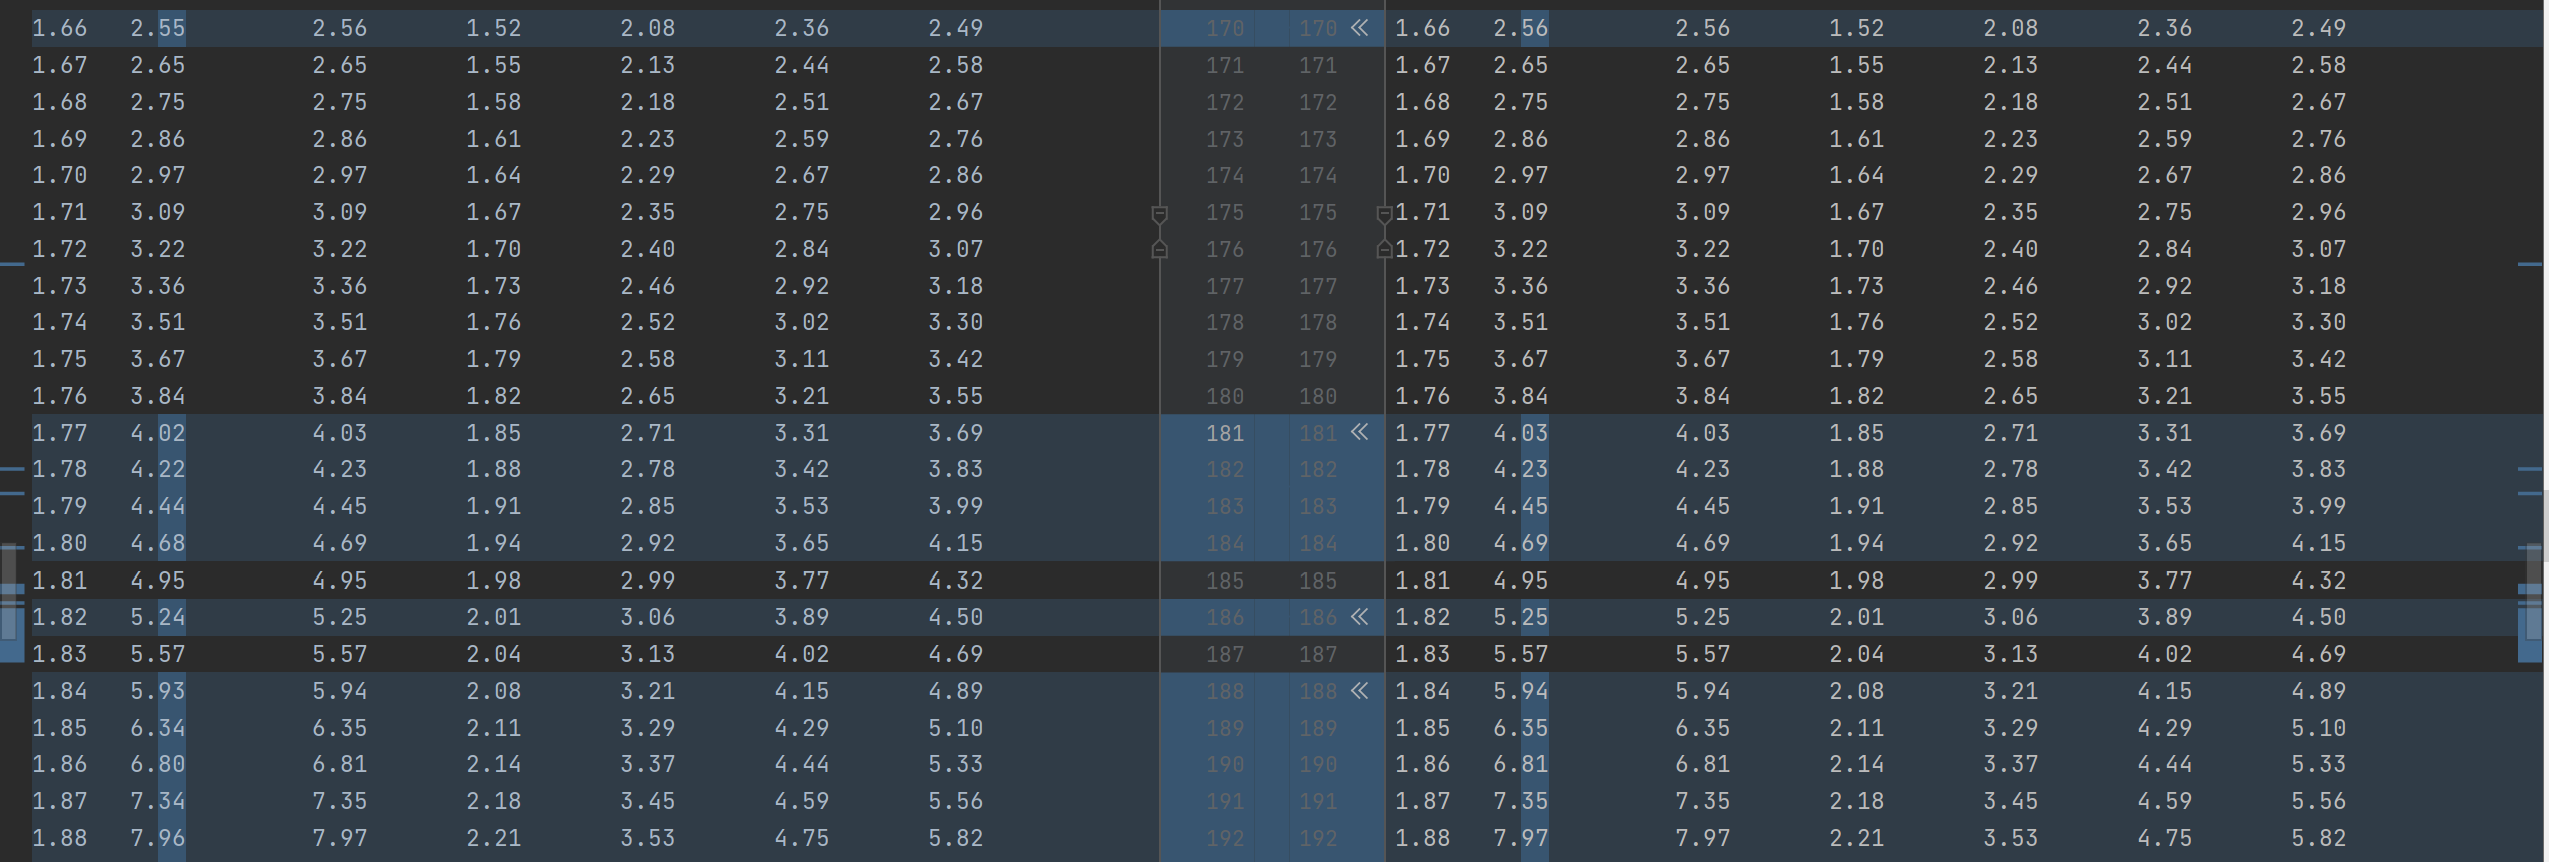
\includegraphics[scale=0.45]{img/differences}\label{fig:differences}

На рисунке видно, что результаты, полученные методом Эйлера на одних и тех же аргументах, но с разным шагом, начинают сильно отличаться при x=1.77, поэтому именно это значение и выбрано в качетсве максимального.

\chapter{Ответы на вопросы}

\textbf{1. Укажите интервалы значений аргумента, в которых можно считать решением заданного  уравнения каждое из первых 4-х приближений Пикара. Точность результата оценивать до второй цифры после запятой. Объяснить свой ответ.}

i-е приближение Пикара можно считать решением уравнения до тех пор, пока совпадают результаты для i-го и (i+1)-го приближений до второго знака после запятой.

Основываясь на таблице результатов:

\begin{itemize}
	\item 1-ое приближение можно считать решением на отрезке [0, 0.84];
	\item 2-ое приближение можно считать решением на отрезке [0, 1.06];
	\item 3-ое приближение можно считать решением на отрезке [0, 1.37];
	\item для определения промежутка, на котором 4-ое приближение можно считать решением, необходимо использовать 5-ое приближение. При его расчете происходит ошибка OverflowError: int too large to convert to float: second\_mult += (chisl / znam)
\end{itemize}


% При данном шаге будут анализироваться значения.
% будем постепенно уменьшать шаг и сравнивать результаты для разных приближений.

\textbf{2. Пояснить, каким образом можно доказать правильность полученного результата при фиксированном значении аргумента в численных методах.}

Путем уменьшения шага для того же метода. Если при меньшем шаге этим же методом получен примерно такой же результат, значит и при большем шаге был получен корректный ответ.

Рассмотрим, например, значение функции при x=1.

По Эйлеру: 
\begin{itemize}
	\item при шаге=$10^{-1}$ y=0.29, 
	\item при шаге=$10^{-2}$ y=0.34, 
	\item при шаге=$10^{-3}$ y=0.35, 
	\item при шаге=$10^{-4}$ y=0.35. 
\end{itemize}

По Рунге-Кутта: 
\begin{itemize}
	\item при шаге=$10^{-1}$ y=0.35, 
	\item при шаге=$10^{-2}$ y=0.35. 
\end{itemize}

Таким образом, правильным ответом является y=0.35, причем при вычислении по Рунге-Кутта можно остановиться на шаге $10^{-1}$, при вычислении по Эйлеру -- на шаге $10^{-3}$

\textbf{3.  Каково значение решения уравнения в точке x=2, т.е. привести значение u(2)}


\begin{equation}
	u(2) \approx 317.72
\end{equation}

\textbf{4. Дайте оценку точки разрыва решения уравнения.}

На рисунке \ref{fig:plot2} приведен график функции в диапазоне [-2.0001; 2.0001].

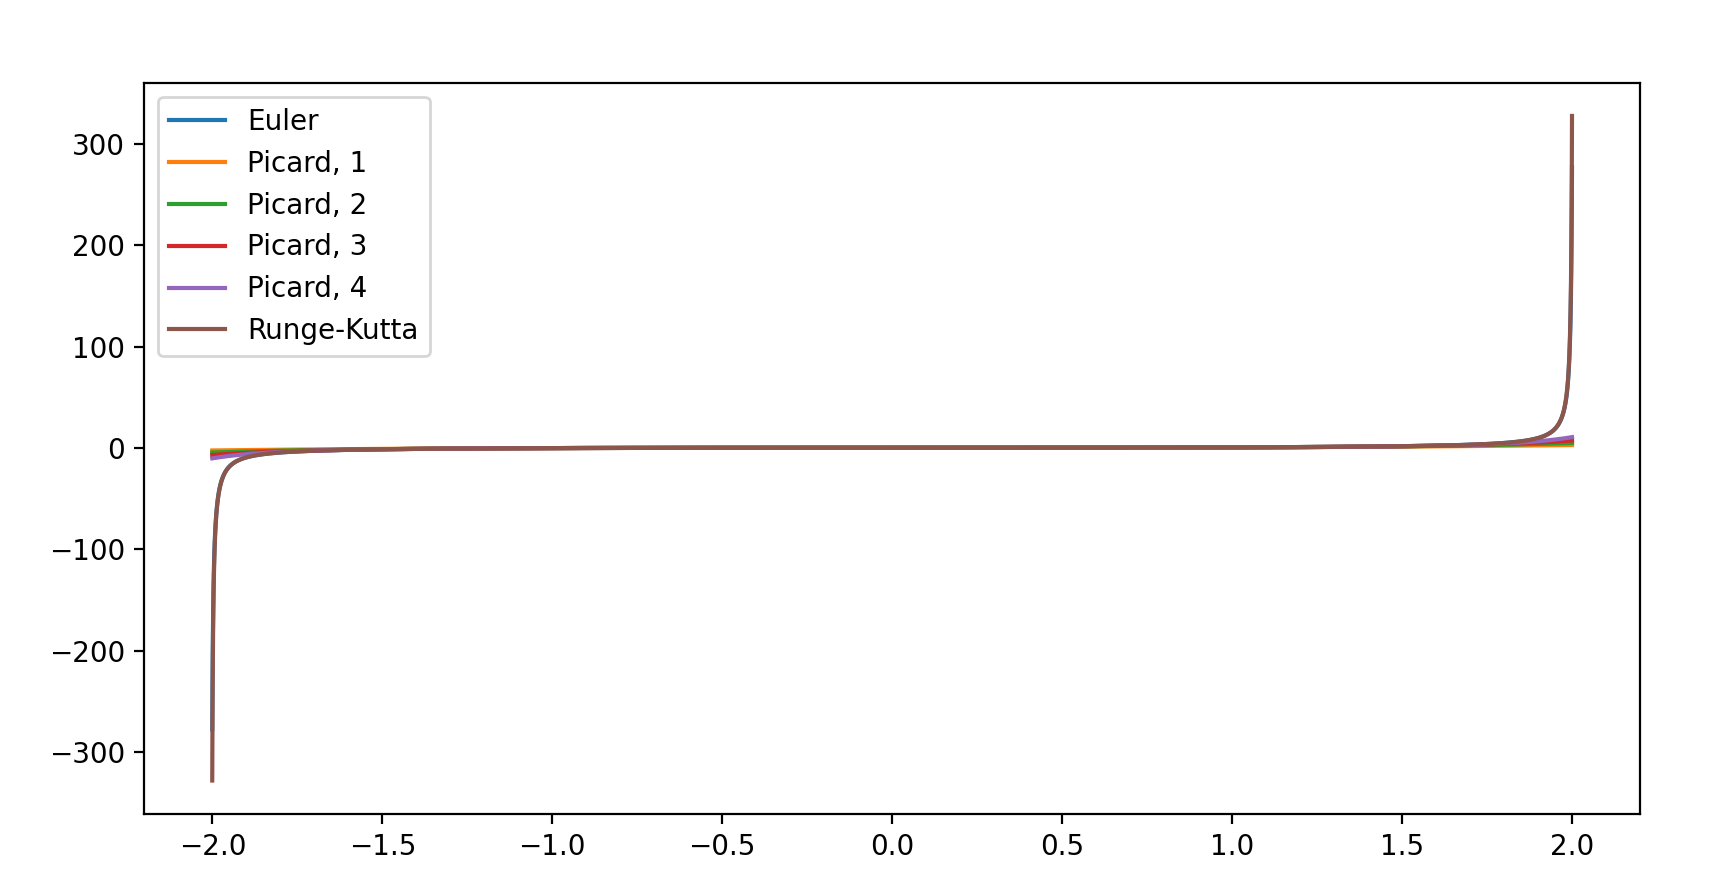
\includegraphics[scale=0.6]{img/plot2}\label{fig:plot2}

По графику видно, что x=-2 и x=2 являются точками разрыва (2 рода) решения уравнения, так как численные методы Эйлера и Рунге-Кутта асимптотически растут при приближении аргумента к этим значениям справа и слева, соответственно.

\textbf{5. Покажите, что метод Пикара сходится к точному аналитическому решению уравнения:}

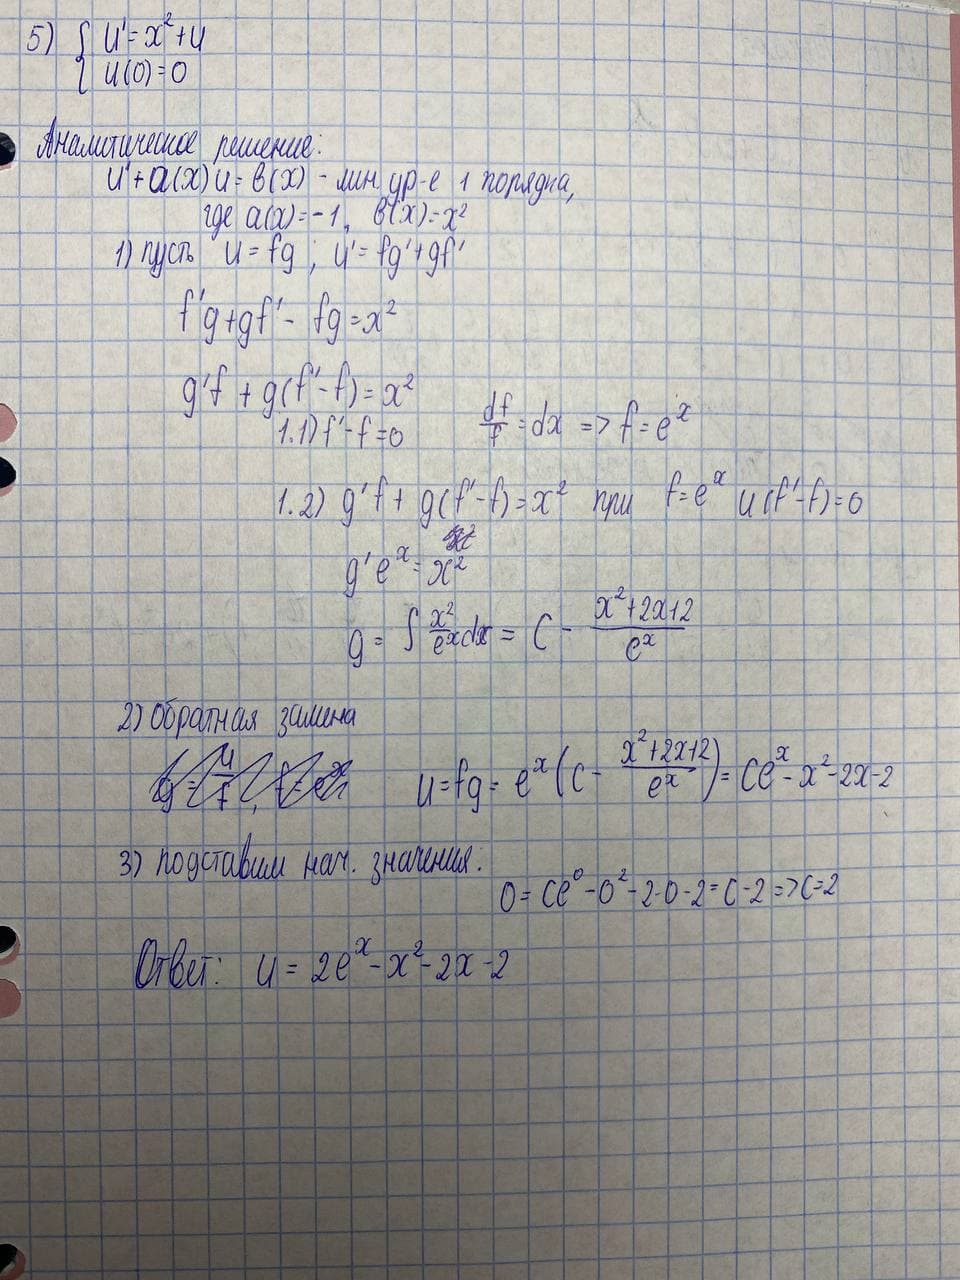
\includegraphics[scale=0.8]{img/2}\label{fig:2}

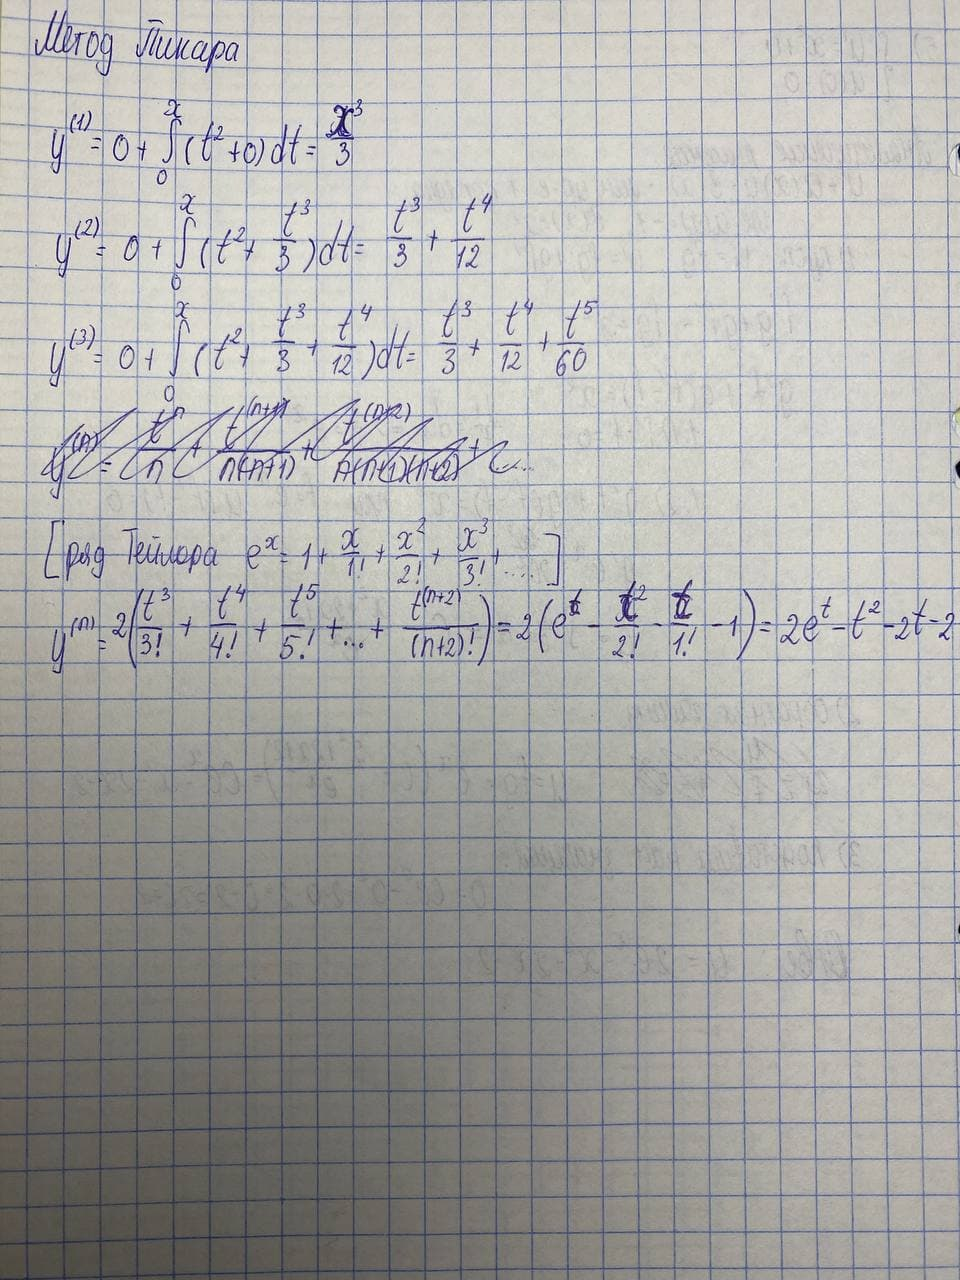
\includegraphics[scale=0.8]{img/1}\label{fig:1}



	\bibliographystyle{utf8gost705u}  % стилевой файл для оформления по ГОСТу
	
	\bibliography{51-biblio}          % имя библиографической базы (bib-файла)
	
	
\end{document}
